

% -------------------------------------------
\section{Introduction}


\subsection{What is NEMO?}
NEMO is a web application for assisting an analyst in understanding contagion processes
and in establishing causality.
It has several features to query and visualize networks, subnetworks, and their properties. A list of features provided by NEMO is summarized in Figure~\ref{fig:user-features}

\begin{figure}[H]
\centering
%\label{fig:ebola-kshell-not-effective}
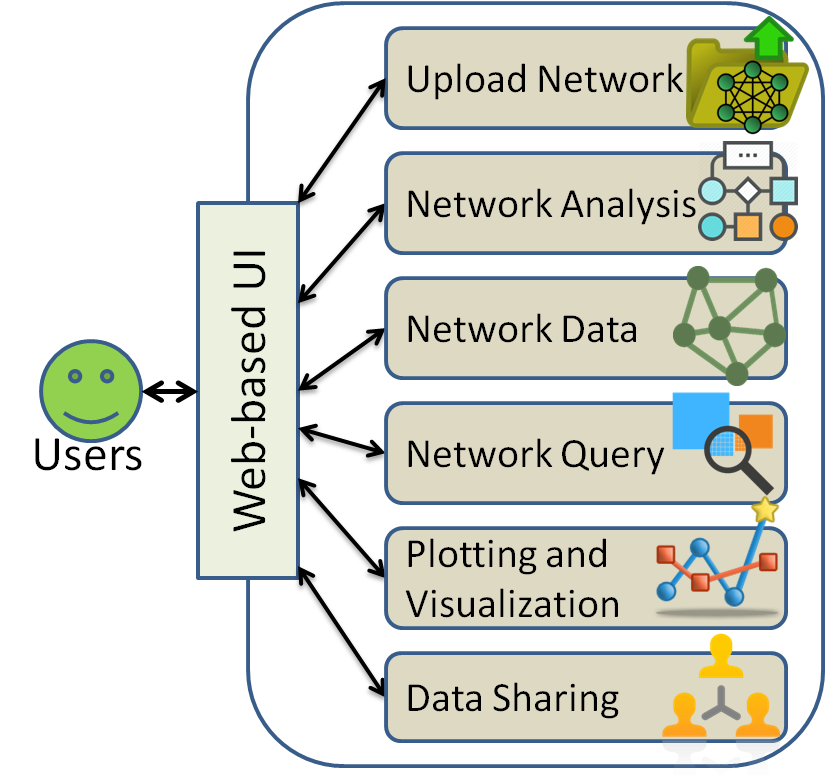
\includegraphics[trim = 0.0in 0.0in 0.0in 0.0in,scale=0.4]{user-features}
\caption{
Features of the NEMO system.
}   %   
\label{fig:user-features}
\end{figure}

\subsection{Features}

\begin{itemize}
\item Exposes the MARS network repository, with the ability to filter and search for networks.
\item Exposes MARS network query service. Users can interactively run queries against network data and download the query results.
\item Analysis of network data using MARS workflow service.
\item Generates publication-quality graphics while interactively explore the data.
\item Network visualization using gephi service.

\end{itemize}




